\chapter{Theory}


\section{Single particle motion in an EM field}

The Lagrangian for a relativistic particle in an electromagnetic field with the potentials $\Phi$ and $\mathbf{A}$ is given by

\begin{equation}
L(\mathbf{r},\mathbf{v},t) = - mc^2 \gamma^{-1}+q \mathbf{v}\cdot\mathbf{A} - q \Phi,
\end{equation}
where $m$ is the mass of the particle, $\gamma$ the relativistic Lorentz factor and q the charge.

To obtain the equation of motion (EoM) we use the Euler-Lagrange equation

\begin{equation}
\frac{\mathrm{d}}{\mathrm{d}t} \frac{\partial L}{\partial \mathbf{v}} - \frac{\partial L}{\partial \mathbf{r}} = 0.
\end{equation}

With $\mathbf{A} = \mathbf{A}(\mathbf{r},t)$, $\Phi = \Phi(\mathbf{r},t)$ and $\gamma^{-1} = \sqrt{1-(v/c)^2}$ and applying the Euler-Lagrange equation this becomes

\begin{equation}
\frac{\mathrm{d}}{\mathrm{d}t} \left[\mathbf{p}+q\mathbf{A}\right]-\left[q\nabla\left( \mathbf{A} \cdot \mathbf{v}\right) - q\nabla \Phi \right] = 0,
\label{Theory:Eqns:EoMLorentzRaw}
\end{equation}
where $\mathbf{p} = \gamma m \mathbf{v}$ is the relativistic momentum.

Now using $\frac{\mathrm{d}}{\mathrm{d}t} = \frac{\partial}{\partial t} + \mathbf{v} \cdot \nabla$ and the vector identity $\nabla \left(\mathbf{v}\cdot\mathbf{A}\right) = (\mathbf{v}\cdot\nabla)\mathbf{A} + \mathbf{v}\times(\nabla\times\mathbf{A})$ this becomes:

\begin{equation}
\frac{\mathrm{d}}{\mathrm{d}t}\mathbf{p} = q\left(\mathbf{v} \times \nabla \times \mathbf{A}-\frac{\partial \mathbf{A}}{\partial t} - \nabla \Phi\right).
\label{Theory:Eqns:EoMLorentz}
\end{equation}

With the definitions of the electric field $\mathbf{E}$ and the magnetic field $\mathbf{B}$ in terms of the potentials  $\Phi$ and $\mathbf{A}$


\begin{align}
\mathbf{E} &= -\frac{\partial \mathbf{A}}{\partial t} - \nabla \Phi,\\
\mathbf{B} &= \nabla \times \mathbf{A},
\end{align}

the equation of motion takes the familiar shape of the Lorentz force:

\begin{equation}
\frac{\mathrm{d}\mathbf{p}}{\mathrm{d}t} = q \left(\mathbf{E} + \mathbf{v} \times \mathbf{B}\right).
\end{equation}

\subsection{Electron motion in a homogeneous electric field}

Using the previously derived equation for the Lorentz force we can now consider a first simple example. Consider the motion of a single electron in a homogeneous electric field $\mathbf{B} = \mathbf{0}$. The Lorentz equation simplifies to:

\begin{equation}
\frac{\mathrm{d}\mathbf{p}}{\mathrm{d}t} = q \mathbf{E}.
\end{equation}

If we choose the coordinate system such that  $\mathbf{E} =  (E,0,0)^t = E e_x$, we see that the momentum of the electron is unchanged in the other two directions, $\mathrm{d}p_x/\mathrm{d}t = \mathrm{d}p_y/\mathrm{d}p_y = 0$. In x-direction the electron however feels a constant force $qE$ accelerating it further and further. 

Let us assume a field strength $E = 100\,\mathrm{MeV/m}$, then the electron will have gained an energy of $100\,\mathrm{MeV}$ after $1\,\mathrm{m}$. After $1\,\mathrm{km}$ it would have gained already $100\,\mathrm{GeV}$ and so on. If we double the field strength, we only need half of the distance to reach the same energy. We just built ourselves a linear electron accelerator! In reality most accelerating structures are not based on static electric fields any more but on matched alternating fields. The principal idea, however, remains the same and the energy gain scales linearly with field strength and the distance over which the particle experiences this field. This is also the motivation and the appeal of plasma based accelerators: plasmas for example can sustain arbitrarily high electric field strengths and some of the accelerating fields measured so far reached an excess of $100\,\mathrm{GeV/m}$ (REF) - we just managed to save us quite some space!

\EliasComm{add diagram of particle acceleration like in between two plates.}

\subsection{Electron motion in a homogeneous magnetic field}

The energy of electrons in wakefield experiments can be determined in experiment using an electron energy spectrometer based on magnetic dispersion. The electrons are deflected using a dipole magnet and detected on a scintillating screen.

In order to understand the fundamental relations this method is based on, the motion of a single electron in a homogeneous magnetic field is considered and analytically solved: first for a motion completely within the magnetic field, then the case of an electron passing through a region of a homogeneous magnetic field of finite extent, but also without considering fringe fields or gradients. In reality, the magnetic fields are measured or simulated and particle tracked using numerical methods.
\vspace{\baselineskip}

Firstly, consider the motion of a single electron in a homogeneous magnetic field extending over the entire region of interest. The equation for the Lorentz force simplifies with $\mathbf{E} = \mathbf{0}$ to:
\begin{equation}
\frac{\mathrm{d}\mathbf{p}}{\mathrm{d}t} = q \mathbf{v} \times \mathbf{B},
\end{equation}

or in terms of the relativistic momentum $\mathbf{p} = \gamma m \mathbf{v}$

\begin{equation}
\frac{\mathrm{d}\mathbf{p}}{\mathrm{d}t} = \frac{q}{\gamma m} \mathbf{p} \times \mathbf{B}.
\end{equation}

Note that in this case the purely magnetic Lorentz force does not do any work. The instantaneous rate of work (power) is $P = \mathbf{F} \cdot \mathbf{v}$, where the force $\mathbf{F}$ is through virtue of the cross product always orthogonal and the dot product vanishes.

We choose the coordinate system such that $\mathbf{B} = (0,0,B)^t = B e_z$. The momentum vector is simply $\mathbf{p} = (p_x,p_y,p_z)^t$.
This then gives us the differential equations:

\begin{align}
\dot{p_x} &= \frac{qB}{\gamma m} p_y\\
\dot{p_y} &= - \frac{qB}{\gamma m} p_x\\
\dot{p_z} &= 0
\end{align}
which gives us

\begin{align}
\ddot{p_x}  &= - \left(\frac{qB}{\gamma m}\right)^2 p_x\\
\ddot{p_y}  &= - \left(\frac{qB}{\gamma m}\right)^2 p_y
\end{align}
which can be solved by a periodic motion of type $p_x(t) = C \sin(\omega t) + D \cos(\omega t)$ with $\omega = qB/\gamma m$. 

$\mathbf{p_\perp}$ be the momentum vector of the particle perpendicular to the magnetic field lines and $\mathbf{p_\parallel}$ the component parallel to the magnetic field (z). Assume initial conditions $p_x(t=0) = |\mathbf{p_\perp}| = p_\perp$ and $p_y(t=0)=0$. We get these equations for the momenta:

\begin{align}
p_x(t) &= p_\perp \cos(\omega t)\\
p_y(t) &= - p_\perp \sin(\omega t) 
\end{align}
The solution for the z-motion is trivial $p_z = p_{z,0}$.

or in terms of the trajectories with $x(0) = 0, y(0) = p_\perp/qB, z(0) = 0$
\begin{align}
x(t) &= \frac{p_\perp}{q B} \sin(\omega t)\\
y(t) &= \frac{p_\perp}{q B} \cos(\omega t)\\
z(t) &= \frac{p_{z,0}}{\gamma m} t
\end{align}

The motion of the electron consists of two decoupled motions: one at the constant, initial velocity parallel to the magnetic field vector in z, the second motion is a circular motion in the x-y plane. This is called a cyclotron motion. For now we will ignore the dissipation of energy in form of radiation due to the acceleration of the electron and accept the result that the Lorentz force conserves the total momentum and energy of the particle in this case.
\vspace{\baselineskip}

The radius of the circular motion of the electron, called the Larmor radius, depends on the total momentum in the x-y plane and the field strength: 
\begin{equation}
r_{Larmor} = |\mathbf{p}_\perp|/eB,
\end{equation}
where $e$ is the charge of the electron and $\mathbf{p}_\perp$ is the component of the momentum vector $\mathbf{p}$ that is perpendicular to the field component of the magnetic field.
\vspace{\baselineskip}

Now consider an external magnetic field restricted to a circle of radius $r_b$ embedded in an otherwise completely field-free region. The following derivation is based on Stuart Mangles' (Imperial College) PhD thesis.
\begin{align}
\mathbf{B} &= B e_z \, &r \leq r_b,\nonumber \\
&= 0 &r > r_b
\end{align}

The angular deflection of a particle in this case can be solved analytically using simple geometry.

\begin{figure}
\centering
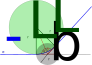
\includegraphics[width=0.5\columnwidth]{elecspec.pdf}
\caption{Visualisation of an electron deflected in a homogeneous circular magnetic field (grey) with radius $r_b$. The larger green circle indicates the Larmor radius, determining the electron trajectory (blue) from the point of entry into the field (A) to its exit point (C) resulting in a total deflection $\theta$.}
\end{figure}

Drawing the circular field region for the magnetic field and the electron entering the field, one can then graphically indicate its Larmor radius, equivalent to its expected motion for the region with the constant B-field. The angles in this constellation are determined using the trigonometric relation that the angles in a triangle have to add up to $\pi$:
\begin{equation}
2 \alpha + \theta = \pi,
\end{equation}
where $\theta$ is the deflection angle and $\alpha$ the angle indicated in the graphic (see figure).

Relating this to the angles to substitute $\alpha$:
\begin{equation}
\tan \alpha = \frac{r_L}{r_b},
\end{equation}
and then expressing this into parameters we can measure in experiment we reach
\begin{align}
\tan \frac{\theta}{2} &= \frac{r_b}{r_L},\nonumber\\
&= \frac{e B r_b}{p_\perp}.
\end{align}

In a typical LWFA experiment $p_\perp$ will be dominated by the component in the laser propagation axis. 

\subsection{Electron in a cylindrically symmetric electric field}

\EliasComm{Maybe move this and the next section to Betatron radiation?}

Now let us assume an electron in a cylindrically symmetric electric field that allows for oscillation. The previously discussed case of a particle in a homogeneous magnetic field corresponds to the motion in a magnetic spectrometer or a circular accelerator.
A field as discussed now is a similar case to a plasma channel or an electron in a wakefield oscillating and generating betatron radiation.


The electron is relativistic and moves in the longitudinal direction. The field structure is cylindrically symmetric around its propagation axis.

As previously we will use a Lagrangian. We ignore any vector potential contributions and only use a scalar potential.

The Lagrangian of this scenario is described by

\begin{equation}
L(\mathbf{r},\mathbf{v},t) = - m_e c^2 \gamma^{-1} - q \Phi
\end{equation}
where $\Phi$ is the scalar potential describing the electrostatic field of the channel.

The scalar potential is the solution matching the radially/cylindrically symmetric Poisson equation

\begin{equation}
\frac{1}{r} \frac{\partial}{\partial r} \left(r \frac{\partial \phi}{\partial r}\right) = \frac{- e (n_0 - n_e)}{\epsilon_0}
\end{equation}

The solution is 
\begin{equation}
\phi = -\frac{(n_0 - n_e) e r^2}{4 \epsilon_0}
\end{equation}

In the extreme case of a completely evacuated channel, $n_e \rightarrow 0$, $\phi = -n_0 er^2/(4\epsilon_0)$.

As before $\mathbf{E} = - \nabla \phi$ and in this case $E_r = - \partial_r \phi$.

The equation of motion for the radial motion is then

\begin{equation}
\frac{d}{dt} \mathbf{p} = - \frac{e^2 n_0}{2 \epsilon_0} r
\end{equation}

Assume there is no axial acceleration field. Assume the radial component of the velocity is small compared to c and the longitudinal component be close to c. $\dot{\gamma}$ is then close to zero. $\mathbf{p} = \gamma m_e \mathbf{\dot{r}}$

The equation then takes the shape of a harmonic oscillator

\begin{equation}
\ddot{r} = - \frac{e^2 n_0}{2\epsilon_0 m_e \gamma} r = - \omega_\beta^2 r
\end{equation}

with a frequency we will call the betatron frequency $\omega_\beta$.

\subsection{Electron in a cylindrically symmetric electric field with axial field}

\EliasComm{Maybe move this section to Betatron radiation?}

Now in addition to the previous case we will add an axial field in the longitudinal (direction of electron propagation). This comes closer to the reality of a wakefield accelerator.
The electric field component shall now be $E_z$, with z being the longitudinal axis.
This gives us an extra term $\frac{\partial \phi}{\partial z} = - E_z$.

The Euler-Lagrangian now has two equations of motions.

Firstly, as before
\begin{equation}
\frac{d}{dt} (\gamma m_e \dot{r}) = \frac{\partial }{\partial r} L = -\frac{e^2 n_0}{2\epsilon_0} r
\end{equation}

Secondly the z-component
\begin{equation}
\frac{d}{dt} (\gamma m_e \dot{z}) = \frac{\partial }{\partial z} L = e E_z = const.
\end{equation}

This time the change in momentum in time is not negligible and we have to expand the brackets.

Radial component:
\begin{equation}
\dot{\gamma}m_e \dot{r} + \gamma m_e \ddot{r} = - \frac{e^2 n_0}{2 \epsilon_0} r
\end{equation}

Axial component is equal to a constant so simply by integrating
\begin{equation}
\gamma m_e \dot{z} = - e E_z t + const.
\end{equation}

If we assume that the electron is very relativistic $\dot{z} \rightarrow c$, so $\dot{\gamma} = eE_z/m_e c$ nad

\begin{equation}
\gamma \beta_z \approx \gamma = - \frac{e E_z t}{m_e c} + \gamma_0 \beta_0,
\end{equation}

where $\gamma_0 \beta_0$ are the initial conditions.

Combining both results and keeping the same assumptions:

\begin{equation}
eE_z \dot{r} + (eE_z t + \gamma_0 \beta_0 m_e c) \ddot{r} = - \frac{e^2 n_0 c}{2 \epsilon_0} r
\end{equation}

Abbreviating some terms....

\begin{equation}
(At + B) \ddot{r} + A \dot{r} + C r = 0
\end{equation}

\begin{equation}
r(t) = \frac{\pi \sqrt{CB}}{A} r_{\beta 0} \left[ J_1 \left( 2 \sqrt{CB}/A \right) Y_0 \left(2 \sqrt{C (B+At)}/A\right) - Y_1 \left(2\sqrt{CB}/A\right)J_0\left(2\sqrt{C(B+At)}/A\right)\right]
\end{equation}
with the initial conditions $r(t=0) = r_{\beta 0}$ and $\dot{r}(t=0) = 0$. 


\subsection{Electron motion in a monochromatic plane EM wave}

Taking the equation of motion (EoM) in terms of the potentials $\mathbf{A}$ and $\Phi$ as given in equation \eqref{Theory:Eqns:EoMLorentz} on page \pageref{Theory:Eqns:EoMLorentz}:

\begin{equation}
\frac{\mathrm{d}}{\mathrm{d}t}\mathbf{p} = q\left(\mathbf{v} \times \nabla \times \mathbf{A}-\frac{\partial \mathbf{A}}{\partial t} - \nabla \Phi\right).
\end{equation}

Now using the convective derivative and the vector identity $\mathbf{v} \cdot \nabla \mathbf{p} = (\nabla \mathbf{p})\cdot\mathbf{v} - \mathbf{v} \times (\nabla\times\mathbf{p})$ again, the total time derivative of the momentum expands:
\begin{equation}
\frac{\mathrm{d}}{\mathrm{d}t}\mathbf{p} = \frac{\partial\mathbf{p}}{\partial t} +(\nabla\mathbf{p})\cdot\mathbf{v} - \mathbf{v}\times(\nabla\times\mathbf{p}).
\end{equation}

With this result the EoM becomes
\begin{align}
\frac{\partial\mathbf{p}}{\partial t} +(\nabla\mathbf{p})\cdot\mathbf{v} - \mathbf{v}\times(\nabla\times\mathbf{p}) &= q\left(\mathbf{v} \times \nabla \times \mathbf{A}-\frac{\partial \mathbf{A}}{\partial t} - \nabla \Phi\right),\nonumber\\
\frac{\partial}{\partial t}\left(\mathbf{p}+q\mathbf{A}\right) +(\nabla\mathbf{p})\cdot\mathbf{v} - \mathbf{v}\times\left(\nabla\times\left(\mathbf{p}+q\mathbf{A}\right)\right) &= - q\nabla \Phi,\nonumber\\
\frac{\partial}{\partial t}\mathbf{u} +(\nabla\mathbf{p})\cdot\mathbf{v} - \mathbf{v}\times\left(\nabla\times\mathbf{u}\right) &= - q\nabla \Phi,
\end{align}
where in the last step we introduced the canonical momentum $\mathbf{u} = \mathbf{p} + q\mathbf{A}$.

Note that
\begin{equation}
(\nabla\mathbf{p})\cdot \mathbf{v} = \frac{1}{m\gamma} \nabla (p^2/2) = \frac{1}{m\gamma}\nabla(\gamma^2/2) = m c^2 \nabla \gamma.
\end{equation}

Using this result to substitute in the previous equation, this can be expressed as
\begin{equation}
\frac{\partial}{\partial t}\mathbf{u} = \mathbf{v}\times\left(\nabla\times\mathbf{u}\right) - \nabla \left(q\Phi + \gamma mc^2\right).
\end{equation}

Taking the curl of this equation results in:

\begin{equation}
\frac{\partial}{\partial t}\nabla\times\mathbf{u} = \nabla\times\left[\mathbf{v}\times\left(\nabla\times\mathbf{u}\right)\right],
\end{equation}
where the second term disappeared as the curl of a gradient is always zero.

This equation shows that if $\nabla \times \mathbf{u}$ is zero initially, it will remain always. The condition is satisfied, for instance, for a plasma at rest before the laser pulse arrives.

Thus, assuming this condition we can write:
\begin{equation}
\frac{\partial}{\partial t}\mathbf{u} = - \nabla \left(q\Phi + \gamma mc^2\right).
\end{equation}

For a medium close to vacuum or an unperturbed plasma one one can assume $\Phi = 0$, resulting in:
\begin{equation}
\frac{\partial}{\partial t}\mathbf{u} =  -\nabla\gamma mc^2.
\end{equation}

In the case of an infinite plane wave the transversal gradient $\nabla_\perp$ is zero.

This means we obtain two separate components:
\begin{align}
\frac{\partial}{\partial t}\mathbf{u}_\perp &= 0,\\
\frac{\partial}{\partial t}\mathbf{u}_\parallel &= \nabla_\parallel \gamma mc^2.
\end{align}

From the perpendicular component we see that the transverse canonical momentum is conserved: $\mathbf{p}_\perp + q\mathbf{A} = 0$. If $q = -e$ and $e\mathbf{A}_\perp = \mathbf{a}_\perp$, then $\mathbf{p}_\perp = \mathbf{a}_\perp$. In terms of the Cartesian coordinates, this means $p_x = a_x, p_y = a_y$.

The parallel component will be considered in the waveframe, using the quasistatic approximation $\frac{\partial}{\partial t} \approx c \frac{\partial}{\partial \xi}$. In this case the spatial component $\xi$ is the direction of propagation, the parallel component, i.e. $\nabla_\parallel = \frac{\partial}{\partial \xi}$. The parallel-component of the vector potential $\mathbf{A}$ is zero, so $u_\parallel = p_\parallel$:

\begin{equation}
\frac{\partial}{\partial \xi}(cp_\parallel - \gamma mc^2) = 0.
\end{equation}

Assuming an unperturbed stationary plasma, the initial conditions are $\gamma = 1$ and $p_\parallel = 0$ and integrating the previous equation gives:
\begin{align}
c p_\parallel - \gamma mc^2 &= - mc^2,\\
cp_\parallel + mc^2 &= \gamma mc^2.
\end{align}

Using $E = \gamma m c^2 = \sqrt{mc^2 + (cp_\parallel)^2 + (cp_\perp)^2}$ and substituting, one obtains an expression for $p_\parallel$:

\begin{equation}
p_\parallel = \frac{1}{2} mc a^2,
\end{equation}
where $a^2 = p^2_\perp$.

Normalising this result by $mc$ we now have:

\begin{align}
p_x &= a_x,\\
p_y &= a_y,\\
p_z &= \frac{1}{2} a^2_z.
\end{align}

In normalised units $\mathbf{p} = \gamma \mathbf{v}$ and this can be written as:

\begin{align}
\gamma \frac{\mathrm{d}x}{\mathrm{d}t} &= a_x,\\
\gamma \frac{\mathrm{d}y}{\mathrm{d}t} &= a_y,\\
\gamma \frac{\mathrm{d}z}{\mathrm{d}t} &= \frac{a^2}{2}.
\end{align}

Changing from $t$ to proper time $\tau$, we transform via $\mathrm{d}\tau = \gamma^{-1}\mathrm{d}t$, simply giving the equation of motions in term of $\tau$:

\begin{align}
\frac{\mathrm{d}x}{\mathrm{d}\tau} &= a_x,\\
\frac{\mathrm{d}y}{\mathrm{d}\tau} &= a_y,\\
\frac{\mathrm{d}z}{\mathrm{d}\tau} &= \frac{a^2}{2}.
\end{align}

Let us assume a laser field with linear polarisation in $x$, described by the vector potential
\begin{equation}
\mathbf{a} = a_0 \cos(\omega \tau)\mathbf{e}_x,
\end{equation}
where $\mathbf{e}_x$ is the unit vector in the x-coordinate. 

\begin{figure}[h]
\centering
	\includegraphics[width=0.49\columnwidth]{figeight_lab.pdf}
	\includegraphics[width=0.49\columnwidth]{figeight_drift.pdf}
\caption{Electron motion in an infinite, linearly polarised, plane EM wave in the lab frame (left), normalised by $a_0/k$ in x and $a^2_0/k$ in z, with the wavenumber $k = \omega/c$. On the right the figure-of-eight motion in the drift frame.}
\label{Theory:Figs:FigureOfEight}
\end{figure}

Using this explicit vector potential and integrating the equation of motions, results in:

\begin{align}
x(\tau) &= \frac{c a_0}{\omega}\sin(\omega \tau),\\
y(\tau) &= 0,\\
z(\tau) &= \frac{c a^2_0}{4}\left(\tau + \frac{1}{2\omega}\sin(2\omega\tau)\right),
\end{align}
where we chose the initial conditions $x(0)=y(0)=z(0)=0$ and returned to non-normalised units.

The electron is performing a periodic oscillation around the z-axis, whilst the motion in the z-axis is composed of a constant drift and another oscillation (see figure \ref{Theory:Figs:FigureOfEight} (left)). This is commonly referred to as the `figure-of-eight' motion, which becomes more evident in the drift frame (see figure \ref{Theory:Figs:FigureOfEight} (right)). For $a_0 \leq 1$ the motion in z is suppressed and the motion of the electron is dominated by the transverse oscillation. For $a_0 \gg 1$, the motion is predominantly longitudinal.

The extremal values are then 

\begin{align*}
x_{max}(\tau = (2n+1)\pi/2\omega) &= \frac{c a_0}{\omega}\\
z_{max}(\tau = (2n+1)\pi/2\omega) &= \frac{c a_0^2 \pi}{8 \omega} (2n+1),
\end{align*}
with $z_{max}$ being unbound as the electron drifts forwards in the lab frame. The drift velocity is (ADD NUMBER HERE) which shows that particles can be accelerated using this method. For a realistic $a_0$ of NUMBER, this gives us a drift momentum of NUMBER. The energies we can achieve in wakefield acceleration is much larger.



\EliasComm{Add lines to the plot for various $a_0$.}

\subsection{Ponderomotive Force}


In laser wakefield acceleration (LWFA) a high intensity laser pulse propagates through an underdense plasma and drives a wave via the ponderomotive force which is proportional to the gradient of the laser intensity. There exists a variety of derivations. The following derivation is based on Alec Thomas' PhD thesis (Imperial College, 2007) (REF).
\EliasComm{add a reference here.}

We start with the Euler-Lagrange equations after plugging in the Lagrangian in terms of the potentials $\mathbf{A}$ and $\Phi$ as given as intermediate step in equation \eqref{Theory:Eqns:EoMLorentzRaw} on page \pageref{Theory:Eqns:EoMLorentzRaw}:

\begin{equation}
\frac{\mathrm{d}}{\mathrm{d}t} \left[\mathbf{p}+q\mathbf{A}\right]-\left[q\nabla\left( \mathbf{A} \cdot \mathbf{v}\right) - q\nabla \Phi \right] = 0.
\end{equation}

This can be written in terms of the normalised quantities
\begin{align}
\mathbf{a} &= -q \mathbf{A}/m_e c,\nonumber\\
\phi &= -q\phi/mc^2,\nonumber\\
\mathbf{v} &\rightarrow \beta = \mathbf{v}/c,\nonumber\\
\mathbf{p} &\rightarrow \mathbf{p}/m c,
\end{align}

resulting in

\begin{equation}
\frac{\mathrm{d}}{\mathrm{d}t} \left[\mathbf{p}-\mathbf{a}\right] - \left(c\nabla \mathbf{a}\right) - c \nabla \phi = 0.
\end{equation}

Now using the canonical momentum $\mathbf{u} = \mathbf{p} - \mathbf{a}$ the time derivative can be re-written and we can also substitute $\mathbf{v} = \mathbf{p}/\gamma = (\mathbf{u}+\mathbf{a})/\gamma$:

\begin{align}
\frac{\mathrm{d}}{\mathrm{d}t}\mathbf{u} &= c\nabla\phi - (c\nabla\mathbf{a})\cdot\frac{(\mathbf{u}+\mathbf{a})}{\gamma},\\
\frac{\mathrm{d}}{\mathrm{d}t}\mathbf{u} &= c\nabla\phi - \frac{1}{\gamma} c \nabla \frac{\mathbf{a}^2}{2}-c\nabla\mathbf{a}\cdot\frac{\mathbf{u}}{\gamma}.
\end{align}

For the situation of an electromagnetic pulse at high frequency $\omega$ of long pulse duration $\tau \gg 1/\omega$ and sufficiently large spot size $w \gg 1/|k|$ in terms of the fast oscillations, fast and slow dynamics can be treated separately.

When averaging over the time of a period $T = 2\pi/\omega$, the terms of linear order $\mathbf{a}$ and the potential $\phi$ amount to zero:

\begin{equation}
\left\langle\frac{\mathrm{d}}{\mathrm{d}t}\mathbf{u}\right\rangle \sim -\left\langle\frac{1}{\gamma}c\nabla\frac{\mathbf{a}^2}{2}\right\rangle,
\end{equation}
which is the ponderomotive force $\mathbf{F}_p$ on on a single electron. Since $\mathbf{F}_p \sim \nabla <\mathbf{a}^2>$, this implies $\mathbf{F}_p \sim \nabla<I>$, i.e. the ponderomotive force pushes electrons away from regions of high intensity and is hence a suitable force to drive LWFA.

\EliasComm{What is the ponderomotive force? Is it not just the electrons gaining mass and oscillating out of the region?}

\iffalse
As the force is essential for the understanding of LWFA it will be derived in the following.

A derivation (Kruer), THIS SECTION NEEDS WORK AS IT IS SO FAR ALMOST 1:1 TAKEN FROM KRUER


HERE A COMMENT WHAT ASSUMED TO TAKE E(x) without the -kx term, as it is a wave actually....

Consider response of a homogeneous plasma to a high frequency field with spatially dependent amplitude $E = E(x) \sin(\omega t)$. We assume $\omega$ is around the electron plasma frequency which in turn is much larger than the frequency of the ion species. The electrons are treated as a fluid and the electron pressure is neglected.

The force equation:
\begin{equation}
\frac{\partial u_e}{\partial t} + u_e \cdot \nabla u_e = - \frac{e}{m} E(x) \sin(\omega t).
\end{equation}

To lowest order $|E|$, $u_e = u^h$ (what is h?)

\begin{equation}
\frac{\partial u^h}{\partial t} = -\frac{e}{m} E(x) \sin(\omega t),\\
u^h = \frac{eE}{m\omega} \cos(\omega t).
\end{equation}

The electrons are oscillating in the electric field. Averaging over the force equation over these oscillations:
\begin{equation}
m \frac{\partial u^s}{\partial t} = -e E^s - m \langle u^h \cdot \nabla u^h \rangle_t,
\end{equation}
where the brackets with index t denote the time average over the high frequency oscillations and $u^s$ is the time average of $u_e$.

Now substituting for $u^h$ from our previous result this gives 

\begin{equation}
m \frac{\partial u^s}{\partial t} = - e E^s - \frac{1}{4} \frac{e^2}{m \omega^2} \nabla E^2(x).
\end{equation}

In addition to the linear term we observe a force that pushes away electrons from regions of high field pressure. The ponderomotive force is proportional to the gradient of the electric field pressure:
\begin{equation}
F_p = - \frac{e^2}{4 m \omega} \nabla E^2 (x)
\end{equation}

When considering this in the relativistic regime, for instance in \cite{Quesnel1998}

in terms of the normalised vector potential
\begin{equation}
F_p = - \frac{1}{2} m_e c^2 \frac{1}{|\gamma|}\nabla \langle a^2 \rangle.
\end{equation}


ANOTHER DERIVATION HERE BASED ON ALEC THOMAS

USE ONE BIT TO EXPLAIN LASER WAKEFIELD ACCELERATION, TAKE THE SECOND TERM TO GO FOR PWFA (PONDEROMOTIVE FORCE MISSING)

\fi



\section{Plasmas}

\subsection{General Properties}

Plasmas are frequently referred to as the `4th state of matter' in addition to the more commonly in daily life encountered matter states solid, liquid and gaseous. Heating up a material at a constant pressure will take it from the solid to the liquid, then to the gas phase and finally will ionize the gas first partially, then completely. The gas is now charged and exhibits interesting collective behaviour due to the dominance of electromagnetic forces whilst upholding quasi-neutrality. This is called a plasma. Sometimes summarised in this definition: ``A quasi-neutral ionized gas that exhibits collective behaviour.'' (REF) However, setting `ionized gas' equal to `plasma' might be a too narrow description as the range of temperature and density scales is very wide for plasmas, including exotic states like the quark-gluon plasma. Although plasmas are probably the most common state of matter in the universe, they barely exists on earth outside of the laboratory environment.
\vspace{\baselineskip}
\EliasComm{if using quote then have to reference.}
\EliasComm{Some examples of plasma states in real life: sun, aurora borealis, wakefields?, neon lamps?}
Two important features of plasma that result in interesting phenomena are quasi-neutrality and collective behaviour.

Whilst a plasma is a charged state, overall approximately equal amounts of opposite charges are available:
\begin{equation}
-e n_e + Z e n_i \approx 0,
\end{equation}
where $e$ is the fundamental charge, $n_e$ the electron number density, $n_i$ the ion number density and $Z$ the charge number of the ions.
Whilst this balance might locally not be true at every moment in time, the mobility of the charges lead to shielding at length scales larger than the so-called Debye length $\lambda_D$:
\begin{equation}
\lambda_D = \left(\frac{\epsilon_0 k_B T_e}{n_e e^2}\right)^{1/2},
\end{equation}
where $\epsilon_0$ is the dielectric constant, $k_B$ the Boltzmann constant and $T_e$ the electron temperature. 

In that sense quasi-neutrality is also a manifestation of `collective behaviour'. Whilst the formation of Debye-spheres is a microscopic effect, the particles can act together on macroscopic scales as well through long range electromagnetic forces to form instabilities and waves. Even small imbalances can give rise to significant responses of the medium. This means that even though plasmas can be modelled as fluids and simulated using hydrodynamic codes, the introduction of electromagnetic forces will give rise to more complex and exotic phenomena than in fluids dominated by gravitational forces.

\subsection{Plasma Formation and Recombination}

Ionisation describes the process of removing an electron from a neutral atom, tipping the charge balance from zero to positive and turning the atom to an ion. Already ionised atoms can be further ionised by stripping more and more electrons from the shells, but this process requires more and more energy as the remainig electrons are bound tighly to the core.

In the context of this work high intensity lasers are used to drive waves in plasmas. A change in the number density of free electrons through ionisation effects can influence the dynamics of the system. The plasma is usually formed by filling a gas compartment or firing a gas jet with a neutral gas, assuming that the laser pulse ionises the gas fully to first approximation.
\vspace{\baselineskip}

There are different mechanisms through which an oscillating laser field ionises a gas. In addition to single photon ionisation, there is multi-photon ionisation \cite{Keldysh1965}, where one electron is excited by absorbing multiple photons before decaying to its original ground state. Another mechanism relies on the collision of electrons and atoms \cite{Latypov1964}. The electric field of the laser can also distort the Coulomb potential of the atom, resulting in a finite probability for electrons to tunnel into the continuum \cite{Perelomov1966}. In the case of very high field strengths, the Coulomb potential might be completely suppressed by the laser field and the atom is immediately ionised: this is called barrier-suppression ionisation \cite{Reiss1970}.
\vspace{\baselineskip}

In the simple example of a hydrogen-like atom in an external electric field $E$, the potential $V$ is given by
\begin{equation}
V(r) = -\frac{Ze^2}{4\pi\epsilon_0 r} - eEr,
\end{equation}
where the position of the maximum potential is given by $r_{max} = (Ze/4\pi\epsilon E)^{1/2}$. Using this result and by setting the height of the barrier to the ionisation potential $V_e$, the electric field required amounts to

\begin{equation}
E = \frac{\pi \epsilon_0 V^2_e}{Ze^3} \approx 173.6 \times \frac{V_e^2 [eV]}{Z}  \mathrm{MV/m},
\end{equation} 

or in terms of intensity using $I = \frac{c\epsilon_0}{2}|E|^2$ in (near) vacuum:

\begin{equation}
I = \frac{c\epsilon_0^3 \pi^2 V^4_e}{2e^6 Z^2} \ approx 4 \times 10^{9} \frac{V_e^4 [eV]}{Z^2} \mathrm{\frac{W}{cm^2}}.
\end{equation}

For hydrogen with $V_e = 13.6\,\mathrm{eV}$ the lower bound intensity required for barrier-suppression ionisation amounts to $1.37 \times 10^{14} \,\mathrm{W/cm^2}$, for helium with $Z=2$ and $V_e = 54.4\,\mathrm{eV}$ the equation gives $I = 8.76\times10^{15}\,\mathrm{W/cm^2}$.
The laser intensities in LWFA experiments routinely reach peak intensities above $10^{18}\,\mathrm{W/cm^2}$. Hence, one can safely assume that ionisation effects are negligible for low $Z$ gases. Higher $Z$ gases like nitrogen are not as easily fully ionized: in hydrogen-like nitrogen the last electron is bound by a potential of $V_e = 667\,\mathrm{eV}$ at $Z = 7$, which translates in intensities required in excess of $10^{19}\,\mathrm{W/cm^2}$. Even very intense laser pulses might struggle to fully ionise a nitrogen gas at all and one can not assume any longer that a fully ionised plasma is in place when the main part of the laser pulse arrives. Typical lasers used for LWFA might struggle to fully ionise nitrogen, but will reach higher degrees of ionisation at peak fields of the laser: this is taken advantage of in an injection method for wakefields called `ionisation injection' (REF). 

\EliasComm{Check that this does not rely on tunnel ionisation.}
\EliasComm{Write about tunnel ionisation.}
\EliasComm{Add sketch of tunnel ionisation and ionisation mechanisms in general.}

Partially ionised plasmas result in a couple of problems: more complex, absorption of X-rays, dampening of particles, scattering? Weaker fields.
\EliasComm{add also some comments on partially ionised plasmas and how they change for instance the absorption of X-rays in this medium.}

\EliasComm{Add sketch of barrier suppression ionisation or all mechanisms in comparison.}

After ionisation the electrons return to the ionic cores of the atom and recombine. During this process called recombination the energy obtained to leave the atom is being released in form of photons again. The wavelength of the radiation is determined by the atom structure and hence characteristic of the material and in case of high Z gases also of the intensity of the interaction. Recombination occurs on a time-scale of XX.

Energy of the photon:
\begin{equation}
E_{ph} = hf = E_{e,kin} + E_{bound}
\end{equation}

\EliasComm{is this true, simple as that?}
\EliasComm{add a diagram to show energy and emission of recombination light.}

The ground level of hydrogen is bound by 13.6 eV corresponding to a photon of wavelength 91 nm (?). The ground level of hydrogen-like helium is bound by a potential $V_e = 54.4\,\mathrm{eV}$, corresponding to a wavelength of 22.8 nm and the first level ionisation level of 24.6 eV corresponds to 50.4 nm.



\subsection{The Plasma Frequency}

The plasma frequency $\omega_p$ is the natural frequency at which electrons will oscillate in a plasma when displaced. It constitutes the typical time scale and the corresponding plasma wavelength $\lambda_p$ the typical length scale of the medium.
\vspace{\baselineskip}

Assume a uniform and neutral plasma, i.e. $n_e = Z n_i = n_{e0}$, where $n_e$ is the electron number density, $Z$ the charge number of the ions, $n_i$ the ion number density, and the initial electric field be $\mathbf{E} = \mathbf{0}$.
Now consider displacing a slab of charge in an arbitrary direction defining an axis that we will call X.

Starting with Gauss' Law:

\begin{equation}
\nabla \cdot \mathbf{E} = \frac{\rho}{\epsilon_0} = \frac{\partial E_x}{\partial x},
\end{equation}
where we used that the displacement is only along $x$, simplifying the nabla operator to a spatial derivative in $x$.

We assume a uniform plasma so the charge density is a constant $\rho = e n_{e0} = const.$. Integrating the previous equation gives an extra factor times the displacement X:
\begin{equation}
E_x = \frac{1}{\epsilon_0} \int^x_0 \rho (x') dx' + E_x(0) = \frac{e n_{e0}}{\epsilon_0} X.
\end{equation}

\begin{equation}
E = \frac{e n_e}{\epsilon_0} X
\end{equation}

If we now consider a force based on this field, we immediately see that this is equivalent to the equation of motion of a harmonic oscillator: 

\begin{equation}
m_e \frac{\mathrm{d}^2 X}{\mathrm{d}t^2} = - \frac{e^2 n_e}{\epsilon_0} X = - \omega^2_p X,
\end{equation}

with the (plasma) frequency

\begin{equation}
\omega_p = \sqrt{\frac{n_{e0} e^2}{\epsilon_0 m_e}},
\end{equation}

and the corresponding wavelength $\lambda_p = 2 \pi c/\omega_p$.

A typical regime wakefield accelerators at a Gemini class laser operate in is at an electron density of around $10^{18} cm^{-3}$. This corresponds to a plasma frequency of around $5.6 \times 10^{13} \,\mathrm{Hz}$ or $\lambda_p \approx 33\,\mathrm{\mu m}$.

\EliasComm{Add sketch on displacing slabs.}

\subsection{The Critical Density}

The critical plasma density $n_c$ is the electron density at which electromagnetic waves can no longer propagate through the plasma. A plasma with a density $n_e < n_c$ is transparent and called `underdense'. For $n_e > n_c$ the plasma is opaque and `overdense'. LWFA requires the laser pulse to propagate through the plasma to drive the wave and hence targets used are typically operating at densities of only a fraction of $n_c$, whilst many ion acceleration mechanisms are based on overdense media.
\vspace{\baselineskip}


\begin{figure}
\centering
\includegraphics[width=0.8\columnwidth]{critical_density.pdf}
\caption{Critical density for wavelengths up to $2 \mu m$. The critical density corresponding to a central wavelength of $0.8 \mu m$, as for the commonly used titanium-doped sapphire (Ti:Sa) lasers, is marked on the graph.}
\end{figure}

\EliasComm{add plot for group velocity vs. density}
\EliasComm{add longer range to include for instance CO2 lasers and mark typical laser frequencies used.}
\EliasComm{write about nonlinear dispersion relation}

Consider a quasi-neutral plasma (charge density $\rho \approx 0$) with a current density $\mathbf{j} = -e n_e \mathbf{v}$, depending on the velocity $\mathbf{v}$ of the electrons in the plasma and the electron density $n_e$. The wave equation for the electric field $\mathbf{E}$ becomes

\begin{equation}
\nabla^2 \mathbf{E} = - \mu e n_e \frac{\partial \mathbf{v}}{\partial t} + \frac{1}{c^2} \frac{\partial^2 \mathbf{E}}{\partial t^2}.
\end{equation}

The acceleration of the electrons is due to the electric field of the wave, i.e. $\partial \mathbf{v}/\partial t = -e\mathbf{E}/m_e$. Now using the solution for a plane wave with $\mathbf{E} = \mathbf{E_0} \exp \left[i (\mathbf{k}\cdot\mathbf{r} - \omega t) \right]$ the dispersion relation is given by $\omega = c k \left(1-\left(\frac{\omega_p}{\omega}\right)^2\right)^{-1/2}$, and hence the group velocity $v_g$ and the phase velocity $v_p$ are given by:

\begin{align}
v_p &= \frac{\omega}{k} = \frac{c}{\sqrt{1-\left(\frac{\omega_p}{\omega}\right)^2}},\\
v_g &= \frac{\partial\omega_L}{\partial k} = c \sqrt{1-\left(\frac{\omega_p}{\omega}\right)^2},
\end{align}
where $\omega$ is the frequency of the electromagnetic wave.

\EliasComm{Add specific example 1m air or vacuum.}

The group velocity reaches zero for $\omega_p = \omega_L$, where $\omega_p$ is the plasma frequency, derived in the previous section and given by $\omega_p = (n_e e^2/\epsilon_0 m_e)^{1/2}$. Solving this for the density, we obtain a relation for the critical density:

\begin{equation}
n_c = \frac{m_e \epsilon_0 \omega^2}{e^2},
\end{equation}
which only depends on the frequency of the incident electromagnetic wave, and so we can write the refractive index $\eta = c/v_p$ in terms of the electron density $n_e$ and the critical density $n_c$:

\begin{equation}
\eta = \sqrt{1-\left(\frac{\omega_p}{\omega}\right)^2} = \sqrt{1-\frac{n_e}{n_c}}.
\end{equation}
\EliasComm{add some comments on the refractive index.}

For $n_e > n_c$, i.e. an overdense plasma, the refractive index is imaginary and the wave becomes evanescent in the medium.

\EliasComm{add some comments here on reflection (plasma mirror).}
\EliasComm{something about absorption of energy in ion acceleration, heating etc.}
\EliasComm{add some explicit curves for transmission/absorption and reflection?}





\section{Wakefield Acceleration}

In the course of the last decades wakefield acceleration has undergone a promising development, strongly influenced by the high intensity lasers available at the time. Creative ideas and schemes were invented to push the boundaries where the lasers available did not reach ideal conditions.

In the early days of wakefield acceleration lasers with femtosecond pulse duration and TW scale were not available.
However, the short duration of the plasma wavelength requires pulse durations on the femtosecond scale.
To overcome this limitation, the beat wave scheme was proposed. Two laser beams at different frequencies are overlapped and start beating in the plasma. If the frequency difference of the two beams is chosen to be the plasma frequency, the beat wave will have the plasma frequency as its beat frequency.
\EliasComm{add some references.}
\EliasComm{add a few lines for self-modulated beams and their recent revival.}

Although the history of wakefield acceleration and its different schemes are certainly fascinating and inspirational for research today, the author will for now focus on laser wakefield acceleration (LWFA) relying on CPA high intensity lasers. %and plasma wakefield acceleration (PWFA), which describes particle-driven wakefield acceleration.
\EliasComm{Nobel prize winning.}

A good and comprehensive overview on this topic explaining the fundamental physics is given in \cite{Esarey2009}, a more recent overview on the progress and status of experiments in the laser wakefield community can be found in \cite{Mangles2016}.

\subsection{Laser Wakefield Acceleration (LWFA)}

In laser wakefield acceleration (LWFA) a short ($\sim 30-50\,\mathrm{fs}$) and intense laser pulse travels through an underdense plasma, driving a plasma wave by pushing the electrons out of its way using the ponderomotive force. Due to the short duration of the laser pulse the ions remain undisturbed and the Coulomb force pulls the electrons back, setting up a density wave. For highly intense pulses $a_0 \sim 1$, the pulse almost completely evacuates the region in its wake with strong longitudinal accelerating fields. This is commonly referred to as the non-linear regime or also the `bubble' regime, where particles can be trapped and accelerated to relativistic energies. The `bubble' regime and the acceleration of quasi-monoenergetic electrons at $100s$ of $\mathrm{MeV} $ has first been reported in 2004 \cite{Mangles2004,Faure2004,Geddes2004}. By now maximum electron energies via LWFA have reached the multi-GeV level in one \cite{Leemans2006} or two stages \cite{Steinke2016,Kim2013}.
\vspace{\baselineskip}

Although supporting several orders of magnitude higher electric fields than conventional RF cavities (for a 3D non-linear wake: $E_{max} = \sqrt{a_0} m_e c \omega_p/e$), the energy and charge of electrons accelerated through the LWFA scheme are limited by several factors, the most important two are the phenomena called \textbf{dephasing} and \textbf{depletion}.
\EliasComm{add some references.}

Firstly, depletion describes the energy loss of the laser pulse as it moves through the plasma and drives the wave. After a certain distance, the depletion length, the pulse is not intense enough any more to drive a stable wave with sufficient field gradients - the cavity collapses. 
The depletion length is given by
\begin{equation}
L_{pd} = 2 \epsilon \left(\frac{a_0}{\delta}\right)^2 \frac{n_c}{n_e} \lambda_p.
\end{equation}

Secondly, in the high field gradients of the wake electrons are relatively quickly accelerated to relativistic energies, reaching velocities close to the speed of light. The driving laser pulse on the other hand propagates through the plasma medium at a group velocity smaller than $c$. The electrons slowly catch up with the driver and leave the accelerating phase of the cavity, this is called dephasing. The dephasing length is the distance over which electrons leave the acceleration phase.

The relativistic electrons are moving close to the speed of light ($\beta_e \rightarrow 1$) whilst the plasma wave moves at a velocity $\beta_p$:
\begin{equation}
\beta_p = \frac{v_g}{c} = \left(1-\frac{n_e}{n_c}\right)^{\frac{1}{2}},
\end{equation}
where $n_e$ is the electron and $n_c$ the critical density.

Using this one can estimate the time it takes the electrons to move out of the acceleration phase of the wave, half the length of the plasma wave:
\begin{equation}
t_d = \frac{\lambda_p}{2c\left(\beta_e-\beta_p\right)}\approx \frac{\lambda_p}{c} \frac{n_c}{n_e}.
\end{equation}
The dephasing length is then 
\begin{equation}
L_{dp} = \lambda_p \frac{n_c}{n_e}.
\end{equation}

This gives the counter-intuitive result that one has to choose low plasma densities (corresponding to lower field gradients) to accelerate particles to higher energies. In addition, this means that one has to balance the between high charge (requiring high $n_e$) and high peak energy. To solve this dilemma and optimise charge and energy, a variety of injection mechanisms (internal \cite{Faure2006,Geddes2008,Pak2010,Buck2013} and external \cite{Hidding2012b,Steinke2016}) have been proposed. The maximum energy gain $W_{max}$ for a 3D non-linear wake is given by \cite{Lu2006}
\begin{equation}
W_{max} = \frac{2}{3}a_0\left(\frac{\omega_L}{\omega_p}\right)^2 m_e c^2.
\end{equation}


\begin{figure}
\centering
\includegraphics[width=0.9\columnwidth]{wakefield_plot.png}
\caption{Visualisation of the laser wakefield acceleration (LWFA) scheme\protect\footnotemark using simulation data. The high-intensity laser pulse (red) travels at almost the speed of light through the plasma (blue), displacing the electrons in its way and driving a wave. The displaced electrons stream back in the wake of the pulse (white arrow) due to the Coulomb attraction. The area of low electron density and the high density regions (green) form strong accelerating fields (orange-red) in the longitudinal direction.}
\end{figure}

\footnotetext{Image taken from Jason Cole's PhD thesis (Imperial College,2015).}

\EliasComm{make own plot for LWFA.}

Other challenges are related to the guiding of the beam: to access higher intensities the laser has to be focused down further. This, however, leads to a rapidly diverging beam, without maintaining the conditions to drive the wave over a long distance. One solution is given by the response of the plasma itself. The interaction of the intense pulse above a critical power $P_c \approx 17 \omega^2_L/\omega^2_p \,\mathrm{GW}$ with the electrons in the plasma can lead to relativistic self-guiding, guiding the laser pulse over multiple Rayleigh lengths, oscillating around the matched spot size $r_b \approx 2 \sqrt{a_0} \frac{c}{\omega_p}$.


\EliasComm{Deviation dephasing, depletion, etching, self-guiding, wavebreaking}

\EliasComm{Plots to show energy versus year, energy spread and type of injection and whether it holds to the scaling laws.}

\subsection{Injection Mechanisms}

\subsubsection{Wave breaking}

Self injection

\subsubsection{Medium based}

Ionisation injection

Clusters and nano particles

\subsubsection{Density Modulations}

- Shock injection
- Downramp
- Upramp

\subsubsection{Laser-assisted}

\subsubsection{External injection}


\iffalse
\subsection{Plasma Wakefield Acceleration (PWFA)}

In plasma wakefield acceleration (PWFA) the laser driver is substituted by a beam of charged particles, for instance electrons\cite{Chen1985}, positrons\cite{Lee2001} or protons \cite{Caldwell2009}. Although the basic concept of driving the plasma wave remains the same, certain parameters will deviate and lead to interesting properties in comparison to LWFA.
\vspace{\baselineskip}

The first thing to notice is that PWFA has been investigated less exhaustively in experiment and breakthroughs have been achieved just in recent years. This is understandable as high quality relativistic charged particle beams as required for PWFA are only available at large accelerator facilities. After a successful demonstration of energy doubling at the Stanford Linear Accelerator (SLAC) \cite{Blumenfeld2007} the interest of the accelerator community increased significantly. By now major facilities such as CERN (AWAKE) \cite{Gschwendtner2016} and DESY (FLASHForward) \cite{Aschikhin2016} as well as other projects in the planning consider PWFA as part of their agenda.

Why is PWFA so attractive and what are its advantages over LWFA?
\vspace{\baselineskip}

PWFA uses a particle beam to drive a plasma wake and to accelerate particles. So far mainly electrons, positrons and protons have been considered as feasible drivers as they are being generated in sufficiently high quality at major facilities today. The relativistic bunch of charged particles will exhibit a space charge which will push away the mobile part of the plasma driving a plasma wake similar as in the case of LWFA.
However, despite the similar concept several differences are to consider. The driver bunch is a highly relativistic particle bunch: until it loses a fair amount of energy, it will propagate at a velocity close to the speed of light, closer than a laser pulse in the plasma medium. Whilst the bunch sustains such an energy level, it avoids dephasing as in the case of LWFA. When heavy particles such as protons are being used at highly relativistic energies, the depletion through interaction with the electrons in the plasma would be negligible and depletion as limiting factor excluded as well. This shows qualitatively the compelling attraction of PWFA: by choosing the right particles the boundaries as existing in LWFA are not present and energy gains of tens, hundreds or even more GeV seem achievable.

Secondly, the `bubble' following the bunch may have a different shape and geometry sensitive to the space charge and its distribution. This may lead to a more favourable focusing field but could also result in other instabilities.

Thirdly, whilst the mechanisms involved in LWFA in the bubble regime are influenced by a number of non-linear effects affecting the stability, the control over the process in PWFA might be much better, especially as the particle beams used are of excellent stability and quality at these facilities. This might require the use of more sophisticated injection mechanisms though.
\vspace{\baselineskip}

However, PWFA introduces new limitations and problems. Just one to mention here is the transformer ratio $R$ which describes the theoretical maximum how much energy can be transferred from the driver to the witness bunch:

\begin{equation}
R = \frac{E^{witness}_{max}}{E^{driver}_{max}} \leq 2 - \frac{N_{witness}}{N_{driver}}.
\end{equation}

 For a longitudinally symmetric bunch it has been shown to be $2$ at maximum \cite{Ruth1984,Caldwell2009} but research is in progress to overcome this limitation by tailoring the driver, the target and using different injection mechanisms.

\EliasComm{be more specific and include recent results.}
\fi



\section{Radiation Production}

After having considered the motion of a charged particle, in this case an electron, in external fields and also discussed briefly the fundamental processes of QED, we should consider the production of radiation in general and the different processes that bear significance in experiments.

Charged particles always then produce radiation when they are being accelerated.

The classical relativistic description requires using retarded Lienard-Wiechert potentials to account appropriately for causality. The trajectories of the electrons as solved before have to be integrated over. In a later section we will discuss why this treatment also lacks in some extreme cases. 

\subsection{Synchrotron Radiation}

In a synchrotron a charged bunch is constantly redirected to remain on a circular orbit. This redirection is an acceleration and hence results in the emission of radiation.

Assume the charged bunch is moving in one big homogeneous magnetic field ignoring separate acceleration and bending modules.
From the previous treatment we know that the charge will move along a Larmor radius determined by the charge mass ratio and the strength of the field. Relativistic particles have an increased effective mass.

We can take this periodic equation of motion and integrate to obtain a spectrum.

Scalings: Power scales to the power of 4?

Insertion devices:
Instead of bending magnets on one big circular trajectory, force the bunch to oscillate strongly while moving through a series of magnets of alternating polarisation. 

Strongest acceleration at the turning points.
Cone related to gamma factor of electrons.

Wiggler parameter: wiggler and undulator regime.

Coherent and incoherent radiation.

This is using the magnetic (!) field!

\begin{equation}
K = \frac{eB_0}{m_e ck_u} = \frac{e B_0 \lambda_u}{2\pi m_e c}
\end{equation}

\EliasComm{energy loss per turn.}
\EliasComm{sketch on emission and cones.}

\subsection{Betatron Radiation}

Just as the evacuated `bubble' in a wakefield accelerates particles in a similar way as conventional RF cavities would, the generation of X-rays draws another parallel in conventional devices.
\vspace{\baselineskip}

Due to initial transverse momentum on injection, and the focusing and defocusing fields of the cavity, electrons start to oscillate around the central axis. 
The electrons oscillate at the so-called betatron frequency $\omega_\beta$
\begin{equation}
\omega_\beta = \omega_p / \sqrt{2 \gamma},
\end{equation}
which depends on the plasma frequency $\omega_p$ and the energy of the electrons here given by the relativistic Lorentz factor $\gamma$.

\EliasComm{done this derivation earlier and might want to combine sections.}
\EliasComm{add plot to show particle motion either pic or PIC.}

Similarly to electrons in an insertion device (undulator or wiggler) these oscillations lead to the emission of radiation in a narrow forward pointing cone due to the relativistic forward momentum of the particles.
Not surprisingly, the equations describing both processes are very similar.

The collimation depends on $K$, the wiggler parameter (for insertion devices) or betatron strength parameter
\begin{equation}
K = \gamma k_\beta r_\beta,
\end{equation}
where $k_\beta = \omega_\beta / c$ is the wavenumber and $r_\beta$ is the betatron radius, the amplitude of the oscillations. If $K \gg 1$ it is called the undulator parameter.

The radiation generated follows the on-axis synchrotron radiation with a critical energy
\begin{equation}
E_c = \frac{3}{4} \hbar \gamma^2 \omega^2_p r_\beta / c,
\end{equation}
where this energy parameter indicates when approximately half the energy radiated above and below this value.
\vspace{\baselineskip}

The oscillation of the particles and hence the emission of radiation can be enhanced in wakefield experiments by tailoring the wavefront \cite{Mangles2009} or by using different injection mechanisms.
In LWFA betatron radiation typically reaches the soft X-ray regime of a few to tens of keV.

Difference here is that we use an quasi-electrostatic field instead of a magnetic field!


\EliasComm{be more extensive and also include comments about absorption in gases).}

\EliasComm{Include some synchrotron equations}

\EliasComm{Include bits about off-axis injection and polarisation.}

\EliasComm{Include an image of betatron oscillations.}

\EliasComm{Include plots on spectrum on- and off-axis.}


\subsection{Bremsstrahlung}

Charged particles that ... atomic collisions... are being accelerated and radiate.
The radiation emitted is commonly called by its German name `bremsstrahlung', which translates into `braking radiation'.

Also sometimes treated as Compton scattering with a virtual photon (from field of the nucleus).

The process of bremsstrahlung is of interest in this context in two ways:
Firstly, we use the process to generate high-energetic gamma radiation. Relativistic electrons accelerated in a laser wakefield accelerator are collided with a high-Z material to convert efficiently into a collimated burst of X-rays.

Secondly, the generation of radiation from electrons interacting with solids is an ubiquitous source of noise in the experiments described later on.

Differential cross section under Born approximation (see Jackson):

\begin{equation}
\frac{d \sigma}{d (\hbar \omega)} \approx \frac{Z^2 e^6}{12 \hbar \pi^3 \epsilon_0^3 M^2 c^3} \left(1- \frac{\hbar \omega}{E} + \frac{3}{4} \frac{(\hbar \omega)^2}{E^2}\right) \times \left[\ln\left(\frac{2 E (E-\hbar\omega)}{Mc^2\hbar \omega}\right) - \frac{1}{2}\right] \frac{1}{\hbar \omega},
\end{equation}
for $\hbar \omega < E$.

The number of photons hence scales quadratically with the $Z$ of the converter target used. Higher yield however comes at the cost of spatial resolution and a wider cone of radiation due to scattering in the material.

For $\hbar \omega << E$

\begin{equation}
\frac{d^2 \chi_R}{d \omega d \Omega_\gamma} = \left[\frac{3}{2 \pi} \gamma^2 \frac{(1+\gamma^4 \theta^4)}{(1+\gamma^2 \theta^2)^4}\right] \cdot \frac{d \chi_R}{d \omega}
\end{equation}

\EliasComm{Add an explicit plot of the spectrum}
\EliasComm{Add a plot on the diagram.}

\subsection{Compton Scattering}

Classical Compton scattering describes the inelastic scattering of a photon off an electron which is at rest or close to it. Here the photon loses energy to the electron, hence this is called inelastic. In some conventions this interaction might still be referred to as elastic as energy is transferred into kinetic energy from one particle to another and is not dissipated in terms of heat or deformation. The fully elastic process in the low energy limit is Thomson scattering where the incoming photon does not lose any significant amount of energy in the process.

The reaction can be written as follows:

\begin{equation}
\gamma + e^- \longrightarrow \gamma + e^-.
\end{equation}
\EliasComm{Feynman diagram?}

\subsubsection{Kinematics}

\EliasComm{Add a kinematics diagram}

We will treat the electron and the incoming photon both as particles and calculate their final momenta based on energy and momentum conservation in a relativistic framework.
\vspace{\baselineskip}

The electron has a negligible initial momentum $\mathbf{p}_{e,initial} = \mathbf{0}$ and the total energy hence reduces to the rest energy of the electron $E_{e,initial} = m_e c^2$. The subscript $e$ stands for `electron'.
The photon on the other hand has initally a momentum $\mathbf{p}_{\gamma, initial}$ and an energy $E_{\gamma, initial} = p/c = hf$, where $h$ is Planck's constant and $f$ the frequency of the photon. The subscript $\gamma$ represents the photon in this interaction.

Relying on the conservation of energy we can postulate that the sum of energies before and after the interaction have to be equal:
\begin{align}
E_{e, initial} + E_{\gamma,initial} &= E_{e,final} + E_{\gamma,final},\nonumber\\ 
m_e c^2 + h f &= \sqrt{(p_{e,final} c)^2 + (m_e c^2)^2} + h f',\nonumber\\
hf - hf' +m_e c^2 &= \sqrt{(p_{e,final} c)^2 + (m_e c^2)^2},\nonumber\\
\left( hf - hf' +m_e c^2\right)^2 -(m_e c^2)^2 &= (p_{e,final} c)^2.
\end{align}
Here the frequency $f'$ refers to the new frequency of the photon after the interaction.

Similarly we can use momentum conservation to find an expression for the momentum of the electron after the scattering process:
\begin{align}
p_{\gamma, initial} &= p_{e, final} + p_{\gamma, final}\nonumber\\
p_{\gamma, initial} - p_{\gamma, final}c &= p_{e, final}\nonumber\\
(p_{\gamma, initial} - p_{\gamma, final}c)^2 &= (p_{e, final} )^2\nonumber\\
(p_{\gamma, initial})^2 + (p_{\gamma, final})^2 - 2 p_{\gamma, initial}p_{\gamma, final}\cos(\theta) &= (p_{e, final} )^2.
\end{align}

Setting both equations equal we find the familiar equation for the angular dependent change in wavelength of a photon performing Compton scattering with an electron:

\begin{equation}
\lambda_{final} - \lambda_{initial} = \frac{h}{m_e c} (1 - \cos(\theta)) = \lambda_C (1-\cos(\theta)),
\end{equation}
where $\lambda_C = hm_e c$ is the Compton wavelength.

Similarly there is an equation for the emission angle of the electron:
\begin{equation}
\cot(\phi) = (1+\frac{hf}{m_e c^2}) \tan(\theta/2).
\end{equation}

In terms of photon energy we can write
\begin{equation}
E_{\gamma,f} = \frac{E_{\gamma,i}}{1+\frac{E_{\gamma,i}}{m_e c^2}}(1+\cos(\theta))
\end{equation}


These equations describe an angular dependent energy distribution, but not the probability of those interactions.
For this purpose we require the differential cross section for Compton scattering.

\subsubsection{Cross-Section}

The cross section combines the kinematics of the process (as discussed) with the matrix element of the interaction which includes the physics of the interaction.

This derivation is based on Peskin and Schroeder or Schwartz REF.

\EliasComm{differential cross section!!}
\EliasComm{derive KN cross section explicitly}
\EliasComm{polar plot and energy axis}
\EliasComm{add visualisation for ICS (own)}

The spin-averaged Klein-Nishina formula:
\begin{equation}
\frac{\mathrm{d}\sigma}{\mathrm{d}\cos{\theta}} = \frac{\pi \alpha^2}{m^2}\left(\frac{\omega'}{\omega}\right)^2 \left(\frac{\omega'}{\omega} + \frac{\omega}{\omega'}-\sin^2{\theta}\right).
\end{equation}


\begin{equation}
\frac{d \sigma}{d \Omega} = \frac{3}{16 \pi} \sigma_T \left(\frac{E_f}{E_i}\right)^2 \left(\frac{E_i}{E_f} + \frac{E_f}{E_i} - \sin^2 \theta \right)
\end{equation}

For very low energetic photons in the limit $\omega \rightarrow 0$ the cross section simplifies to 
\begin{equation}
\frac{\mathrm{d}\sigma}{\mathrm{d}\cos{\theta}} = \frac{\pi \alpha^2}{m^2} (1 + \cos^2\theta),
\end{equation}
with a total cross section of $\sigma_{total} = 8\pi\alpha^2/(3m^2)$. This is the Thomson scattering cross section.

This cross section and kinematics holds for an electron at rest and a single photon. The cases of one or multiple photons interacting with a relativistic electron are discussed in the following section.

The emission spectrum of Compton scattering at low photon energies is symmetric in the forwards and backwards direction. At increasing photon energies reaching the X-ray and gamma regime the photon is preferentially scattered in the forwards direction.

\EliasComm{Add a low energy differential cross section and spectrum here.}

\subsection{Linear Inverse Compton Scattering}

Laser wiggler. Electric field component, later on at high intensities the magnetic field becomes important as well.

\begin{figure}
\centering
\includegraphics[width=0.8\columnwidth]{ICS_Jason.png}
\caption{Visualisation of inverse Compton scattering (ICS). A relativistic electron is counter-propagated with a laser pulse which gains energy from the interaction due to the relativistic Doppler-effect. Graphics by Jason Cole (Imperial College).}
\end{figure}

\EliasComm{need new ICS visualisation.}

In inverse Compton scattering (ICS) a relativistic electron scatters with one (linear ICS) or multiple photons (non-linear ICS). Whilst in Compton scattering (CS)  momentum is transferred from the photon to the electron (heating), resulting in a longer wavelength of the scattered photon, in ICS the photon gains energy (hence inverse Compton scattering) as it experiences a relativistic Doppler shift.

The photon energies accessible with sufficiently relativistic particles is multiple orders of magnitude higher. In all optical Compton sources \cite{TaPhuoc2012a} relativistic electrons of several hundreds of $\mathrm{MeV}$ have been collided with high-intensity laser pulses, producing tunable X-rays in the $\mathrm{keV}$ \cite{TaPhuoc2012a,Powers2014,Khrennikov2015} to $\mathrm{MeV}$ \cite{Chen2013a,Sarri2014} range with pulse durations of the order of tens of femtoseconds and a micron-scale source size.

In addition to all-optical schemes, it has also been proposed to combine conventional accelerator elements with high-intensity lasers to reach high stability and repetition rates\cite{Seryi2015}.
\vspace{\baselineskip}

The results of a ICS experiment via LWFA at the Astra Gemini facility in the UK are presented later in this report. 

ICS has been widely used in the conventional accelerator community to measure the spin-polarisation of beams.

\subsubsection{Kinematics}

To calculate energy distribution, we can treat this scattering process similarly to the standard Compton scattering we discussed. This requires shifting frames of reference. In the lab frame $S$ quantities will be denoted as before $E, \theta$ and so on. In the rest frame of the electron $S'$ quantities will be denoted as such $E', \theta'$ and so on.

Assume a single relativistic electron beam with a gamma factor $\gamma$ moving in x and a photon of energy $E_{i}$ with an incident angle $\theta_i$.
In the rest frame of the electron the photon experiences a relativistic Doppler-shift. 

\begin{equation}
E'_i = \gamma E_i (1-\mathbf{\beta} \cdot \mathbf{e_k}) = \gamma E_i (1 - \beta \cos\theta) \approx \gamma E_i (1- \cos\theta),
\end{equation}
where we assumed that the electrons are highly relativistic and $\beta \approx 1$.
In a head-on collision ($\theta = \pi$) the photon energy is in the electron rest frame by a factor $2\gamma$ higher.
For $E'_i << m_e c^2$ we are now in the Thomson scattering regime in this frame of reference.

In the rest frame we can now treat this normally for Compton scattering. The photon energies of the scattered photon and the angles follow the previously discussed equations.

\begin{equation}
E'_f = \frac{E'_i}{1+\frac{E'_i}{m_e c^2}(1-\cos\alpha')},
\end{equation}
where $\alpha'$ is the difference between the incident and outgoing angle. As for normal Compton scattering the photon is now losing energy in this frame.

\begin{equation}
\cos \alpha' = \mathbf{n'_f} \cdot \mathbf{n'_i} = \cos \theta'_i \cos \theta'_f + \sin \theta'_i \sin \theta'_f \cos(\phi'_i - \phi'_f)
\end{equation}
with $\phi'$ angles being the azimuthal angles of the photon.

The energies have to be boosted back into the lab frame. This gives another factor amplifying the energy of the photon
\begin{equation}
E_f = E'_f \gamma (1+\beta \cos \theta'_f) \approx E'_f \gamma (1+ \cos \theta'_f)
\end{equation}

From these equations we see that the maximum energy can be achieved in a head-on collision and observing the radiation on-axis.
The photons are boosted by $(2\gamma)^2$ to an energy $E_{f,max} = 2 \gamma E'_f = 2 \gamma E'_i = 4 \gamma^2 E_i$.


\subsubsection{Cross-Section}

The calculation of the cross section follows the same scheme, relying on the quantum-corrected Klein-Nishina equation using the angles and energies in the electron rest frame. The angles corresponding to the cross sections and the solid angles, however, have to be transformed in a similar way.

At $\gamma >> 1$ we will assume that the collisions are always head-on, such that $\sigma' = \sigma$ and we need to only change the solid angle.
Due to the relativistic boost the energy of the photons will look as if $2\gamma$ higher and we will be in the regime where the Klein-Nishina equation already indicates a headlight effect of the radiation being preferably emitted in forwards direction.

\begin{figure}
\centering
\includegraphics[width=.5\columnwidth]{ThomsonScattering.png}\includegraphics[width=.5\columnwidth]{Headlight.png}
\caption{Rest frame and lab frame emission. ICS.}
\end{figure}

\EliasComm{add some parts here from Jason's calculations.}

\EliasComm{add plot for relativistic kinematics.}

\subsection{Nonlinear Inverse Compton Scattering}

\begin{equation}
n\gamma_L + e^- \longrightarrow \gamma + e^-.
\end{equation}

\subsubsection{Kinematics}

Relativistic kinematics is identical for one or several photons as many incoming identical energy photons and one outgoing with n times $\omega$ the energy. When following the kinematics through one arrives at the same equation as previously for the scattering process in the rest frame of the electron

\begin{equation}
E'_f = \frac{n E'_i}{1+\frac{n E'_i}{m_e c^2}(1-\cos\alpha')},
\end{equation}

At laser intensities reaching an relativistic regime $a_0 ~ 0.1$ the equation of motion of the electron starts deviating from a simple up-and-down oscillation due to a longitudinal component. The electrons start performing a figure-of-eight motion with a longitudinal component increasing with $a_0$.
This additional component has two effects:
Firstly, the modification of the equation of motion leads to a redshifting of the spectrum. The energy of the Doppler-shifted radiation is damped to 
\begin{equation}
\hbar \omega' \approx \frac{4 \hbar \omega a_0 \gamma^2}{1+a_0^2/2 + \gamma^2 \theta^2},
\end{equation}
This leads to a downshift and broadening of the radiation.

We solved the equation of motion previously and it follows the relativistic Doppler shift.

\begin{equation}
\omega' = \gamma \omega (1-\beta \cos(\theta)) \approx \omega (1+\gamma^2 \theta^2)/2\gamma
\end{equation}

Secondly, energy is being transferred from this fundamental radiation at $\omega$ to higher order harmonics $\omega_1 = n\omega$, when multiple photons upconvert to one higher energy photon. Since this is a free electron process the harmonics are not restricted to either odd or even numbers but cover both.
Fourier analysis.

The angular distribution of each component is distinct and symmetric, with odd harmonics showing a maximum on-axis and (n-1)/2 lobes on either side and even harmonics having a minimum on-axis and n/2 side-maxima on either side.

\begin{figure}
\centering
\includegraphics[width=.5\columnwidth]{ICS_Redshift.png}\includegraphics[width=.5\columnwidth]{ICS_Redshift2.png}
\caption{Redshift of the fundamental harmonic.}
\end{figure}

\EliasComm{make a plot for the spectrum and correct this spectrum to reflect the spectrum in the lab frame or make notable that this is in the rest frame. Maybe compare the two.}


In the highly nonlinear regime $a_0 \gg 1$ the number of harmonics increases by a factor $a_0^3$ (REF). At the same time each harmonic is spread out due to the longitudinal component which now dominates the electron motion.

The high number of harmonics (hundreds!) and the redshifting of each component transforms the spectrally very peaked spectrum to a broadband source resembling a synchrotron spectrum.

This means to reach higher photon energies a more intense laser is not necessarily the best option as the redshifting appears rapidly along with the harmonics. A more energetic electron provides a redshift-free upshift. If one wants a close to monoenergetic spectrum on top of that linear Compton scattering in the limit $a_0 \rightarrow 0$ is more suitable.

\subsubsection{Cross-Section}

Volkov state, Furry picture, dressed states.

Infinite series of diagrams in this set.

\EliasComm{One, two photon feynman diagrams. Add image of dressed states and series equivalent.}

Models: classical harmonics, polarisation dependency, quantum model.

\subsubsection{Other modifications of the spectrum}

In a real setting the ICS spectrum is modified by several input parameters:
the energy spread of the electron beam will translate to an energy spread in the ICS spectrum.
Short pulse lasers intrinsically require a certain bandwidth are hence not monochromatic. The spread of photon energies modifies the spectrum similarly.
Deviations from a head-on collision have to be considered and also introduce a spread, in particular considering divergence and emittance of the electron beam and the range of angles of the focusing laser pulse with respect to the laser axis.


\section{Radiation Reaction}

\EliasComm{How does radiation reaction compare to the ponderomotive force? It scales with $1/\gamma$ so it is less important in this context but what does it mean?}

The previous sections left out the effect of radiation losses onto the equation of motion of charged particles.
Charged particles emit radiation when being accelerated. The charged particle emitting the radiation loses the energy associated with the photon and is knocked back, adhering to momentum and energy conservation rules. This is called radiation reaction or radiation friction.
Radiation reaction is a very fundamental problem of physics and a universally accepted description does not exist. Each description only exists in a certain limit and is an approximation valid within those limits.

In many cases the radiation losses are small or occur over longer spans of time which means they can be ignored or the detailed physics of radiation reaction is not important. In storage rings of large accelerator and collider facilities radiation losses pose a significant problem as they limit the maximum energy the particles can be accelerated to. The exact dynamics of radiation reaction and the influence on the equation of motion of the particles is not very significant. It suffices to add the average energy lost over the a turn in the storage ring to prop up the system.

Radiation reaction effects become more significant in extreme conditions where ultra-relativistic particles interact with light: in astrophysical phenomena.
These conditions are re-constructed in accelerator facilities interacting ultra-relativistic particles with laser pulses. Radiation reaction was measured, for instance, at SLAC and first measurements have been undertaken at non-conventional accelerators such as the Astra-Gemini laser system at the Central Laser Facility in the UK. This work is part of this thesis.

\subsection{Radiation reaction: classical runaway solutions}

This section is based on Jackson. REF!
One intuitive way to derive an expression for radiation reaction is considering conservation of energy. It is well known that accelerated charges emit radiation which is fairly well characterised in the context of synchrotrons, other circular accelerators or undulator setups. The emitted power follows the Larmor power formula

\begin{equation}
P = \frac{2}{3} \frac{e^2}{c^3} \mathbf{\dot{v}}^2.
\end{equation}

This equation can be used to derive an expression for a radiation force by integration.
The explicit steps can be found in Jackson (Chapter 16, equations 16.7 to 16.8).

The in Jackson called `radiative reaction force' then becomes
\begin{equation}
F_{rad} = \frac{2}{3} \frac{e^2}{c^3}\mathbf{\ddot{v}} = m \tau \mathbf{\ddot{v}}.
\end{equation}

The equation of motion then reads
\begin{equation}
m(\mathbf{\dot{v}}-\tau \mathbf{\ddot{v}}) = \mathbf{F}_{ext}.
\end{equation}

This equation of motion, sometimes referred to as Abraham-Lorentz equation, depends on the second derivative of the velocity in time which results in so-called runaway solutions.
For a vanishing external force, we obtain two solutions for $\mathbf{\dot{v}}$:
\begin{equation}
\mathbf{\dot{v}}(t) = 0 \,or\, \mathbf{a}e^{t/\tau}.
\end{equation}

$\mathbf{a}$ is the acceleration at $t = 0$. If $\mathbf{a} \neq 0$ we run into trouble.

First attempts to simply add radiation reaction as a force onto the Lorentz-force equation resulted in unphysical expressions depending on several derivatives of the velocity. This in the end required knowing about the future to calculate its equation of motion, and led to self-acceleration of the particles in question. These solutions are commonly referred to as 'runaway solutions'.

The relativistic generalisation was found by Dirac renormalising in 4-space. The result is referred to as Lorentz-Abraham-Dirac equation (LAD).

\EliasComm{Remember which metric to use? +--- or -+++}

\EliasComm{Here add some calculations explicitly.}

\EliasComm{Jackson seems to be in cgs. Make sure you know which unit system you work in.}

\subsection{Self-consistent classical description: Landau-Lifschitz}


\EliasComm{Furry picture, treating the laser field as classical external field.}


A first self-consistent solution to including radiation reaction into a classical model was achieved by Landau and Lifschitz (REF).


Problems: energy loss can exceed initial energy. Stochasticity not included.

\subsection{Quantum Corrections}

Quantum parameter eta and chi. $\eta = E_{RF}/E_{crit}$

Limit when quantum effects become more important: energy loss comparable to rest mass of the electron?

With high confidence we know that we require a quantum description of this process.
There are several ways to solve some of the issues of the classical Landau-Lifschitz description.

Critical field for quantum electrodynamics $E_{crit} = 1.38 \times 10^{18}\,\mathrm{V m^{-1}}$

REFS: Chris Ridgers JoP

Corrections regarding spectrum of radiation (cut-off).

Stochasticity.

Semi-classical approach using Gaunt factor.

\begin{equation}
g(\eta) = \frac{\int_0^{\eta/2} F(\eta, \chi) \mathrm{d}\chi}{\int_0 F_{cl}\left(\frac{4\chi}{3\eta^2}\right)} = \frac{3 \sqrt{3}}{2 \pi \eta^2} \int_0^{\eta/2} F(\eta,\chi) \mathrm{d}\chi. 
\end{equation}

Fit for function is (Baier 1991):

\begin{equation}
g(\eta) \approx \left(1 + 4.8(1+\eta)ln(1+1.7\eta)+2.44\eta^2\right)^{-2/3}.
\end{equation}

Assuming local constant cross field approximation (LCFA).
Formation time, coherence time.



Cooling of spectra versus competing processes.




